\subsection{Open Targets}
\label{subsec:ot}

Open Targets is a large--scale, public--private partnership with the aim of generating an informatics platform that utilises genetic germline, genetic somatic, gene expression, literature, pathway, and drug data to link 18,104 genes and diseases to develop a GDA prioritisation \cite{ferrero2017}. The targets could be a genes, transcripts or proteins defined by Ensembl nomenclature. Diseases were described by the \href{https://goo.gl/YvvC8D}{EFO} \cite{experimentalFactorOntology2010}. The evidence is described in the \href{https://goo.gl/CNqAqt}{Open Biomedical AssociatioN} (OBAN) representation \cite{sarntivijai2016}. OBAN is an ontology that represents triple-form entities of \texttt{subject--related--to\_object}. For example, an entity \texttt{disease} is the subject, the relationship \texttt{has\_evidence} and the objects could be entities \texttt{phenotypes} plus the source of evidence for that association

The information obtained from different public domain databases (see Table \ref{tab:ot_db}) was classified into seven different \texttt{data types} (see Data type in Table \ref{tab:ot_db}).

\begin{table}[H]
\centering
    \begin{tabular}{c|c|c|c}
      Data source & Data type & \texttt{evidence\_score} \\
      \hline
      
      \href{https://goo.gl/sfm7CC}{Reactome} & Affected pathway &
      Curator score = \{1,0\} \\
      
      \href{https://goo.gl/egMxCH}{PhenoDigm} & Animal Model &
      Similarity score \cite{PhenoDigm2013} \\
      
      \href{https://goo.gl/A4UjA5}{GWAS Catalog} & Genetic association &
      $ FCS^* \cdot sample\_size \cdot p_{value} $ \\
      
      \href{https://goo.gl/Vavb1L}{EVA} & Genetic association & 
      FCS* \\
      
      \href{https://goo.gl/5SiDMj}{UniProt} & Genetic association &
      Curator score = \{0.5,1\} \\
      
      \href{https://goo.gl/qwDPhK}{Gene2Phenotype} & Genetic association &
      Curator score = 1 \\
      
      \href{https://goo.gl/dXL3jQ}{Cancer Gene Census} & Somatic mutation &
      FCS* \\
      
      \href{https://goo.gl/kTWn6z}{IntOGen} & Somatic Mutation &
      Tumor type category score = \{0.25, 0.5, 0.75\}\\
      
      \href{https://goo.gl/tJ2wzt}{ChEMBL} & Known drug & Clinical phase score = \{0.09, 0.1, 0.2, 0.7, 1.0\} \\
      
      \href{https://goo.gl/P3UAc9}{Europe PMC} & Literature text mining & Confidence score \cite{kafkas2017} \\
      
      \href{https://goo.gl/1eQbbs}{Gene Expression Atlas} & RNA expression & $p_{value} \cdot sample\_size \cdot percentile\_rank $ \\
      
      \end{tabular}
\caption{Data sources for GDA information the Open Targets pipeline. A more detailed explanation of the \texttt{evidence\_score} is described by Koscielny et al. \cite{koscielny2016}. (*) FCS means Functional Consequence Score. Available in the original publication at \href{https://goo.gl/gkvHxK}{Supplementary Table 2. FCS}.\label{tab:ot_db}}.
\end{table}

There are four score that were described as follows:

\begin{table}[H]
\centering
    \begin{tabular}{c|p{12cm}}
      Score & Description \\ \hline
      
      \texttt{evidence\_score} & Comprises the (i) \texttt{frequency}, (ii) \texttt{magnitude}, and (iii) \texttt{confidence} of GDAs \cite{koscielny2016} in Table \ref{tab:ot_db}. E.g. in GWAS Catalog: frequency corresponds to sample size, magnitude to the predicted FCS of the variation, and confidence to a p-value \\ \hline
      
      \texttt{data\_source\_score} & Harmonic sum al all sorted evidence score in descending order \\ \hline
      
      \texttt{data\_type\_score} & Harmonic sum of all scores belonging to the same data type. E.g. the  \texttt{genetic\_association} with the GWAS Catalog, EVA, UniProt, and Gene2Phenotype scores (see Table \ref{tab:ot_db}) \\ \hline
      
      \texttt{overall\_score} & Harmonic sum of all \texttt{data\_type\_score} \\ 
      
      \end{tabular}
\caption{Open Targets scores and their description \label{tab:ot_scores}}.
\end{table}

Why they include \texttt{sample\_size} if the formula of the p-value already includes information about the sample size? The code snippet below in \texttt{Python} will demonstrate it:
\lstinputlisting[language=Python]{data/pval_uncertainty.py}

\subsubsection{Reproduction of pipeline in the paper}
Ferrero et al. code in R version 3.3.0 was versioned using GitHub and is available \href{https://goo.gl/C4cSgQ}{elsewhere}. For more information about the pipeline, please refer to Ferrero el al. \cite{ferrero2017}. The results in this report were obtained using the targets from \href{https://www.cortellis.com}{Cortellis}, provided by Exscientia, and not the ones from PharmaProjects as described in the article \cite{ferrero2017}. Please note that all the results are not displayed here, for a full explanation of the reproduction please download the \href{https://github.com/davidnarganes/iCASErep}{GitHub repository} and compile in LaTeX to generate the PDF version.

\begin{figure}[H]
    \centering
    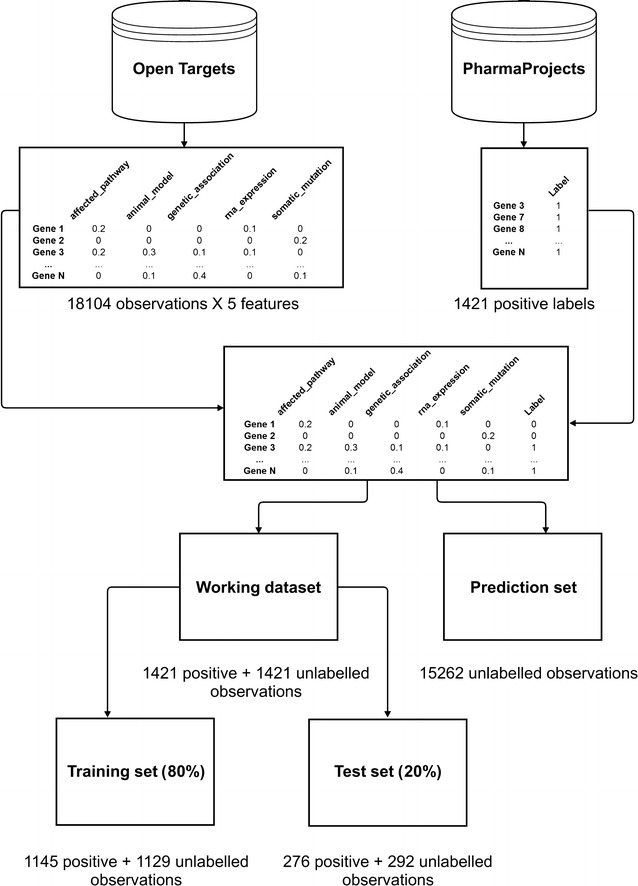
\includegraphics[width=0.5\textwidth]{pics/workflowOpenTargets.jpg}
    \caption{Workflow for the target prediction. While the labels were collected from Informa Pharmaprojects  \cite{pharmaProjects} in the original publication, the results shown here used the targets from Cortellis, provided by Exscientia. The resulting data matrix was split into a \texttt{working set} (1421 positives and 1421 randomly selected unlabelled) and a \texttt{prediction set} (15262 unlabelled genes). The \texttt{working set}, containing both positive and unlabelled observations, was further split into \texttt{training set} and \texttt{test set} to evaluate the performance of the classifier. The \texttt{prediction set} was kept aside and used to perform predictions once all four classifiers was trained}
    \label{fig:ot_workflow}
\end{figure}

Two exploratory analyses were performed: principal component analysis (PCA) (figure \ref{fig:OT_PCA}) and t-Stochastic Neighbourhood Embedding (tSNE) (Figure \ref{fig:OT_tSNE}). Given that the student did not know how these algorithms worked, PCA and the SNE part of t-SNE were coded in Python from scratch (see Annex).

\begin{figure}[H]
\resizebox{\textwidth}{!}{
    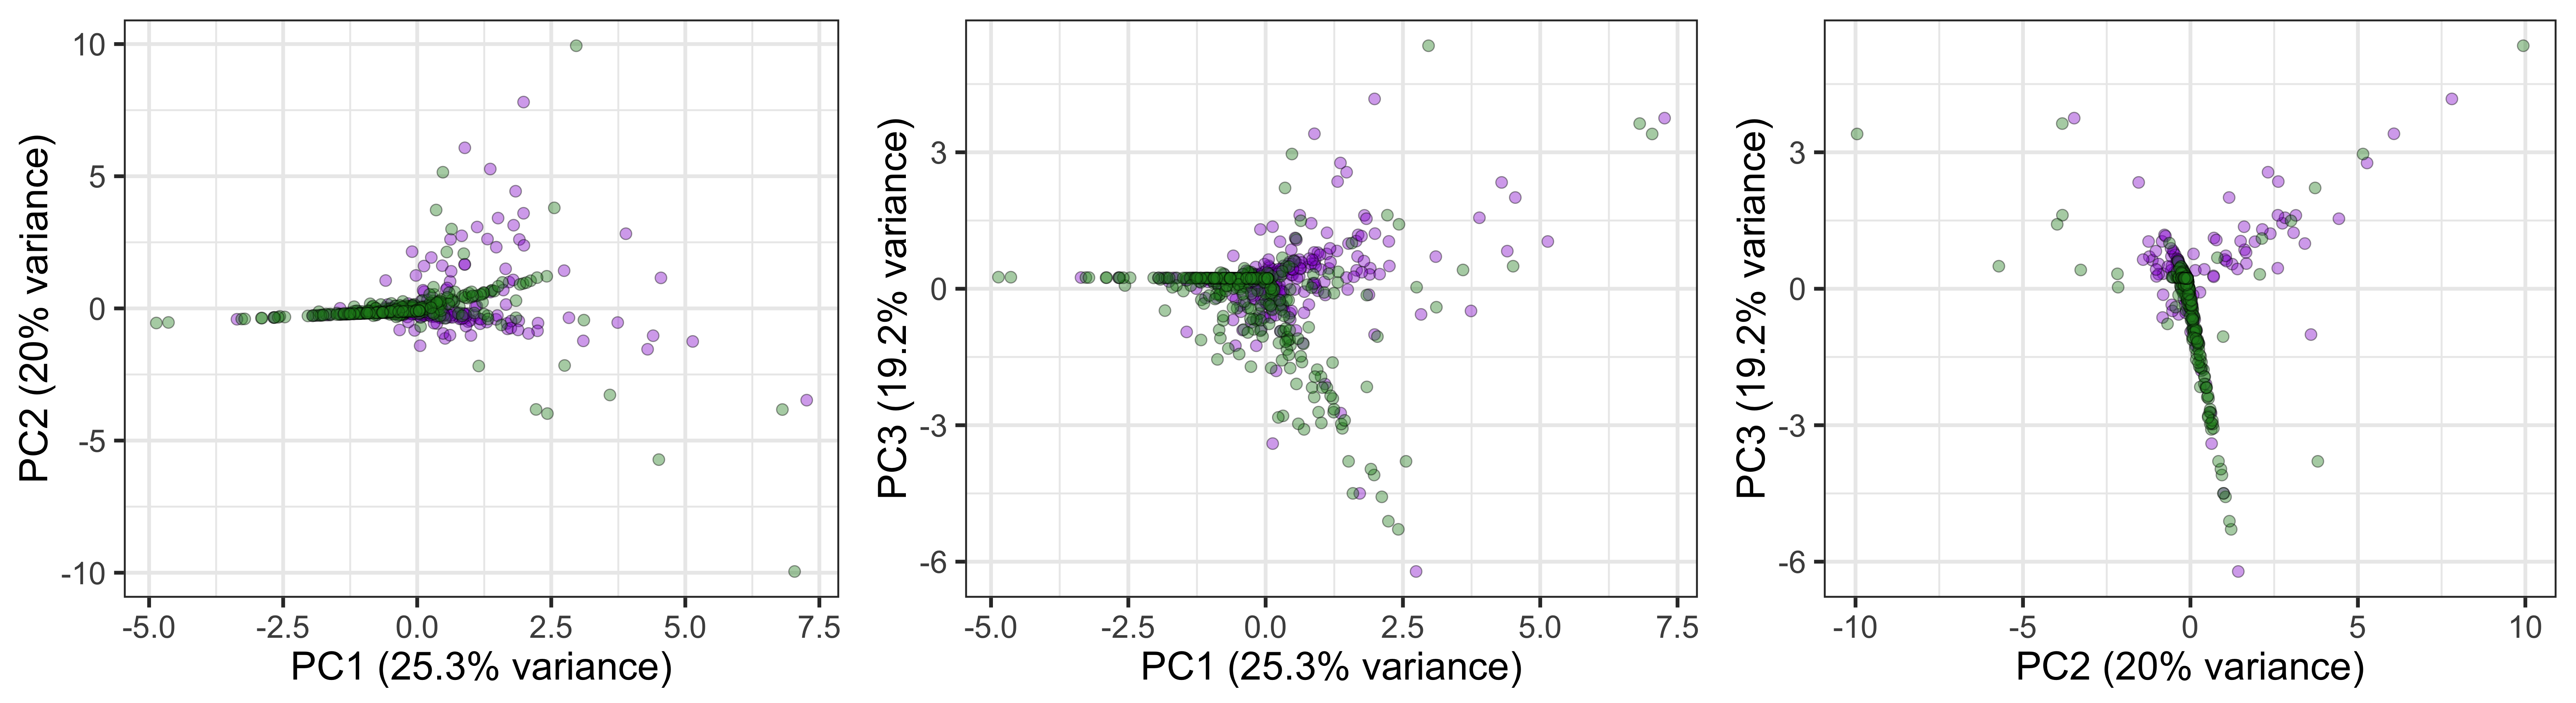
\includegraphics{pics/PCAh.png}}
    \caption{Exploratory data analysis of the \texttt{working set} using PCA for linear dimensionality reduction. Each dot in the two-dimensional space represents a gene and is coloured according to its label (green target, purple non-target)}
    \label{fig:OT_PCA}
\end{figure}

\begin{figure}[H]
\centering
    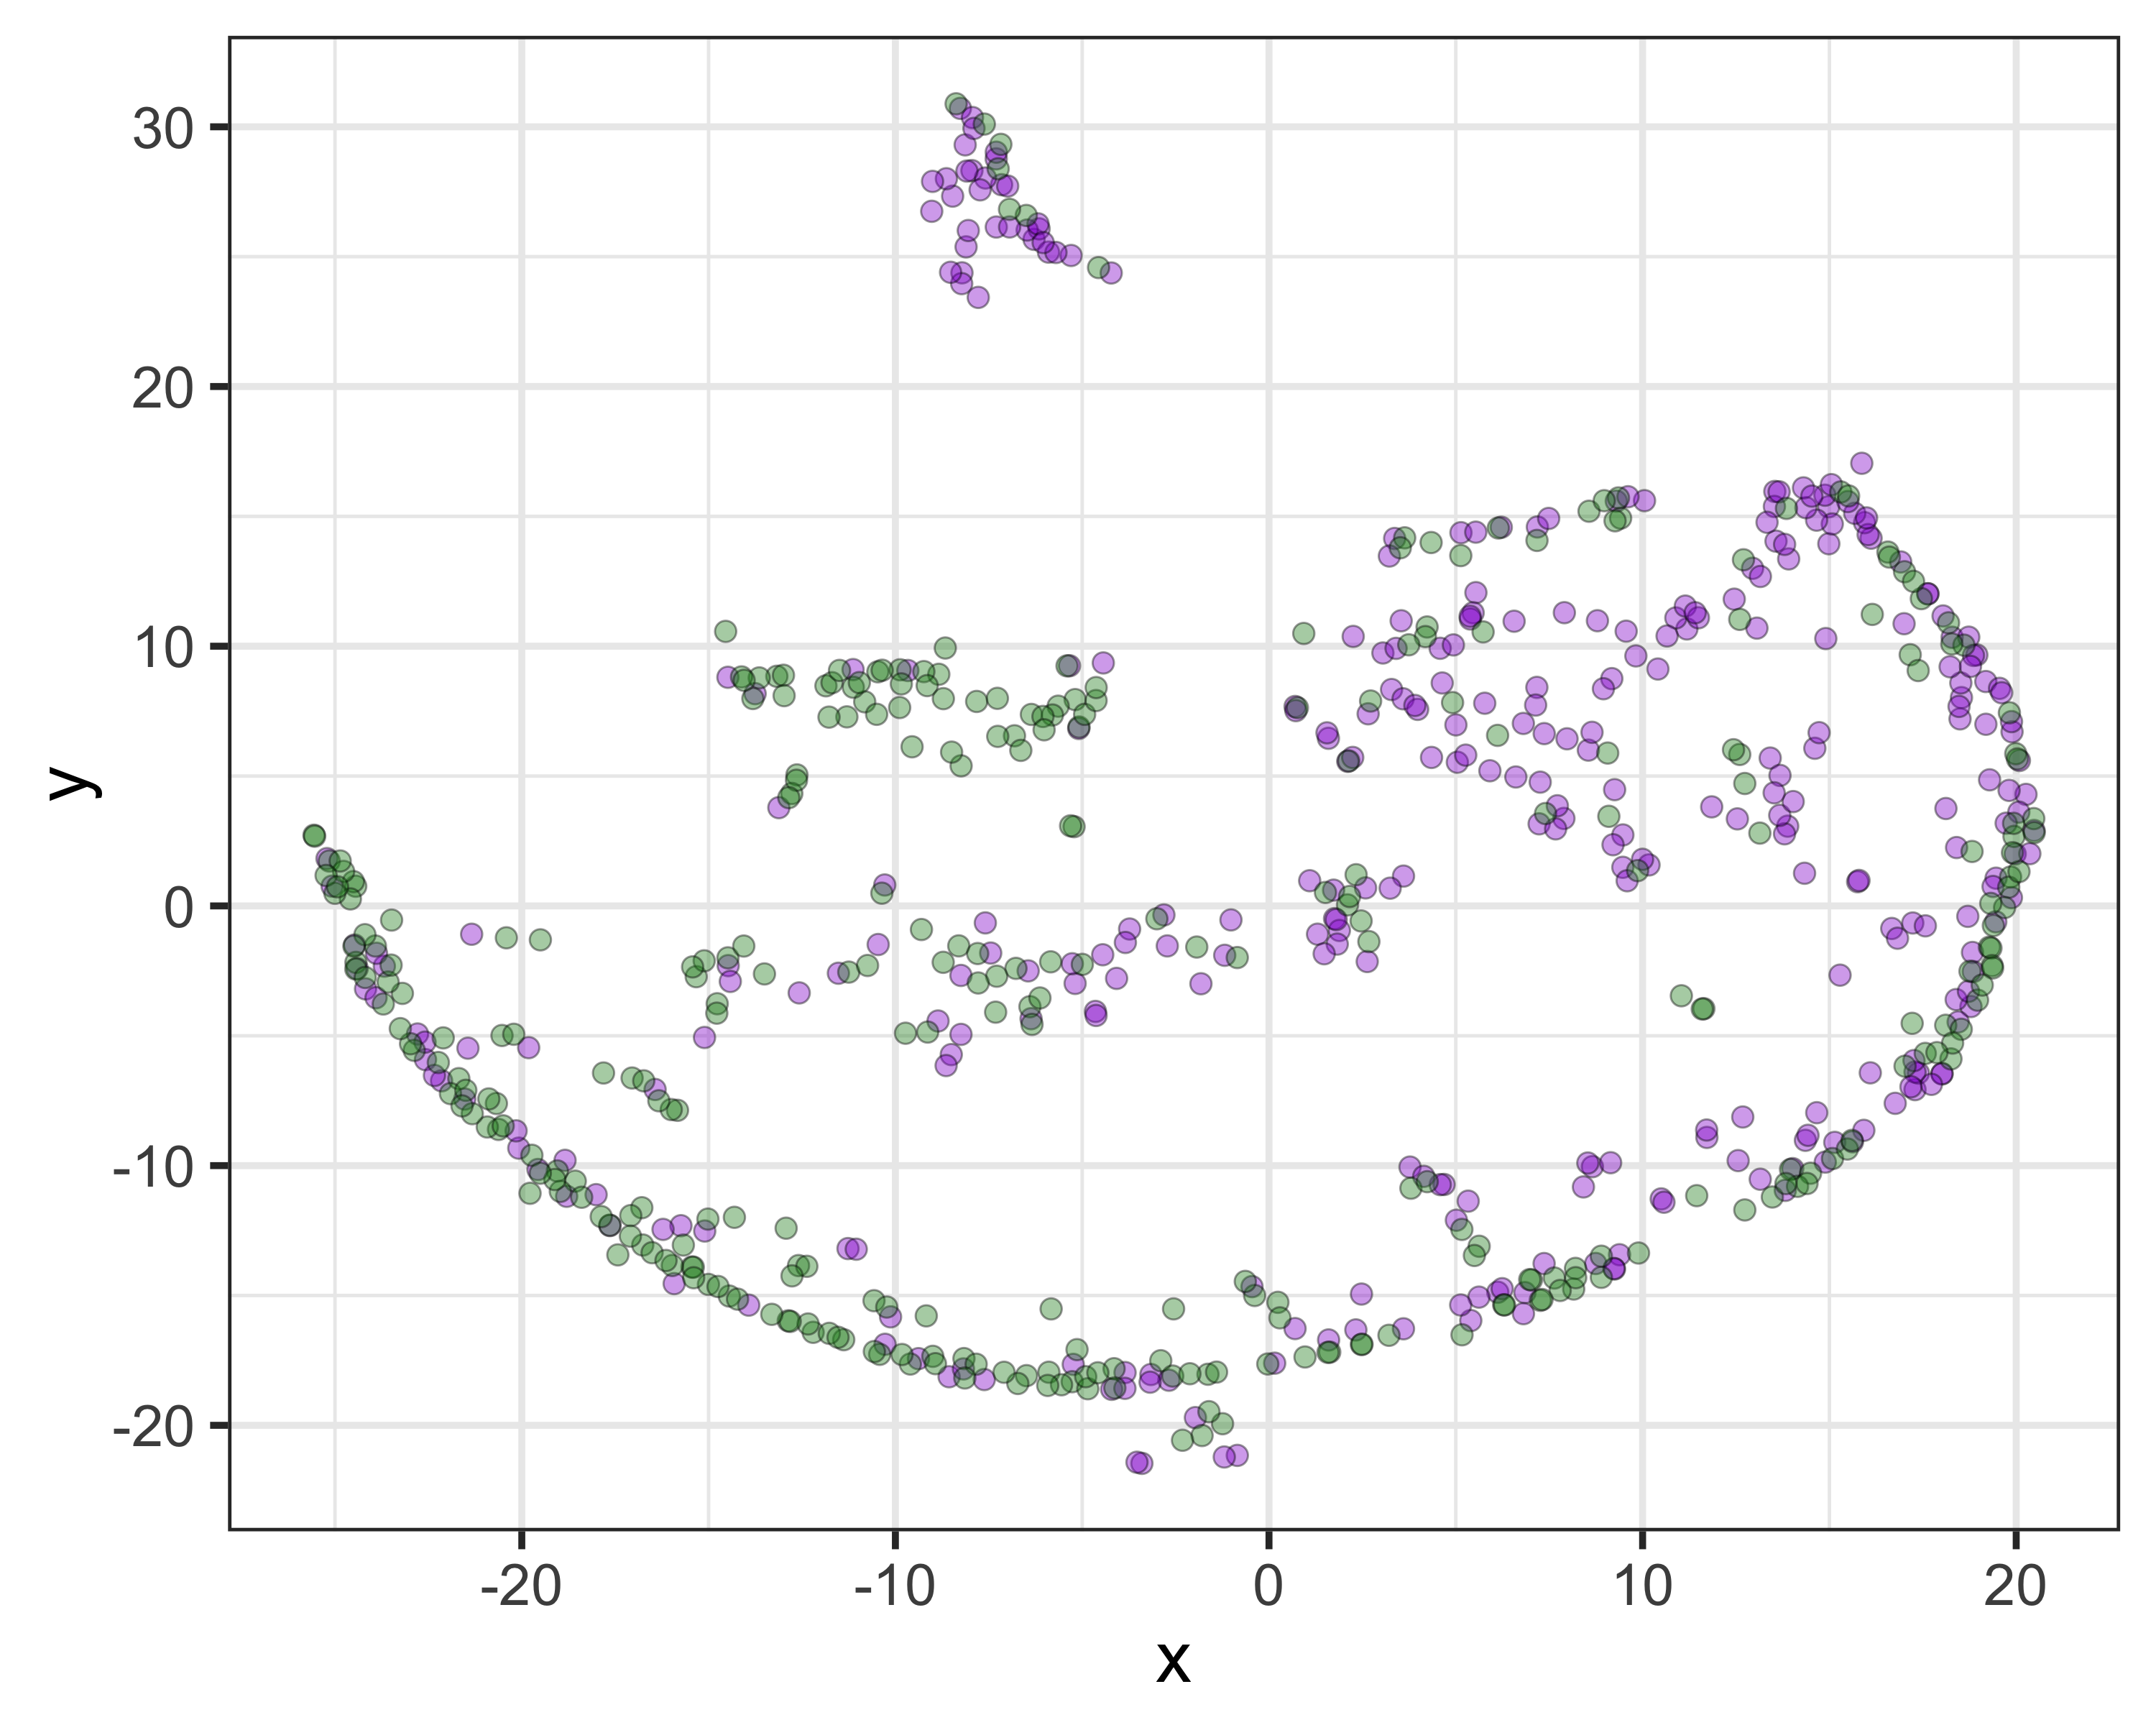
\includegraphics[width=9cm]{pics/tSNE.png}
    \caption{Exploratory data analysis of the \texttt{working set} using dimensionality reduction. The tSNE algorithm for non-linear dimensionality reduction was run a perplexity value of 30 and other default parameters. Each dot in the two-dimensional space represents a gene and is coloured according to its label (green target, purple non-target)}
    \label{fig:OT_tSNE}
\end{figure}

Figure \ref{fig:OT_features} shows the relative importance of each data type whereas Figure \ref{fig:OT_features} represents the classification criteria with a decision tree. In the three approaches, \texttt{animal\_model}, \texttt{rna\_expression} and \texttt{genetic\_association} showed the most informative power. These results are important and will be discussed in Section \ref{subsub:limitations_openTargets}.

\begin{figure}[H]
\subfloat[Feature importance according to Chi Squared test and information gain with the \texttt{working set} \label{fig:OT_features}]{
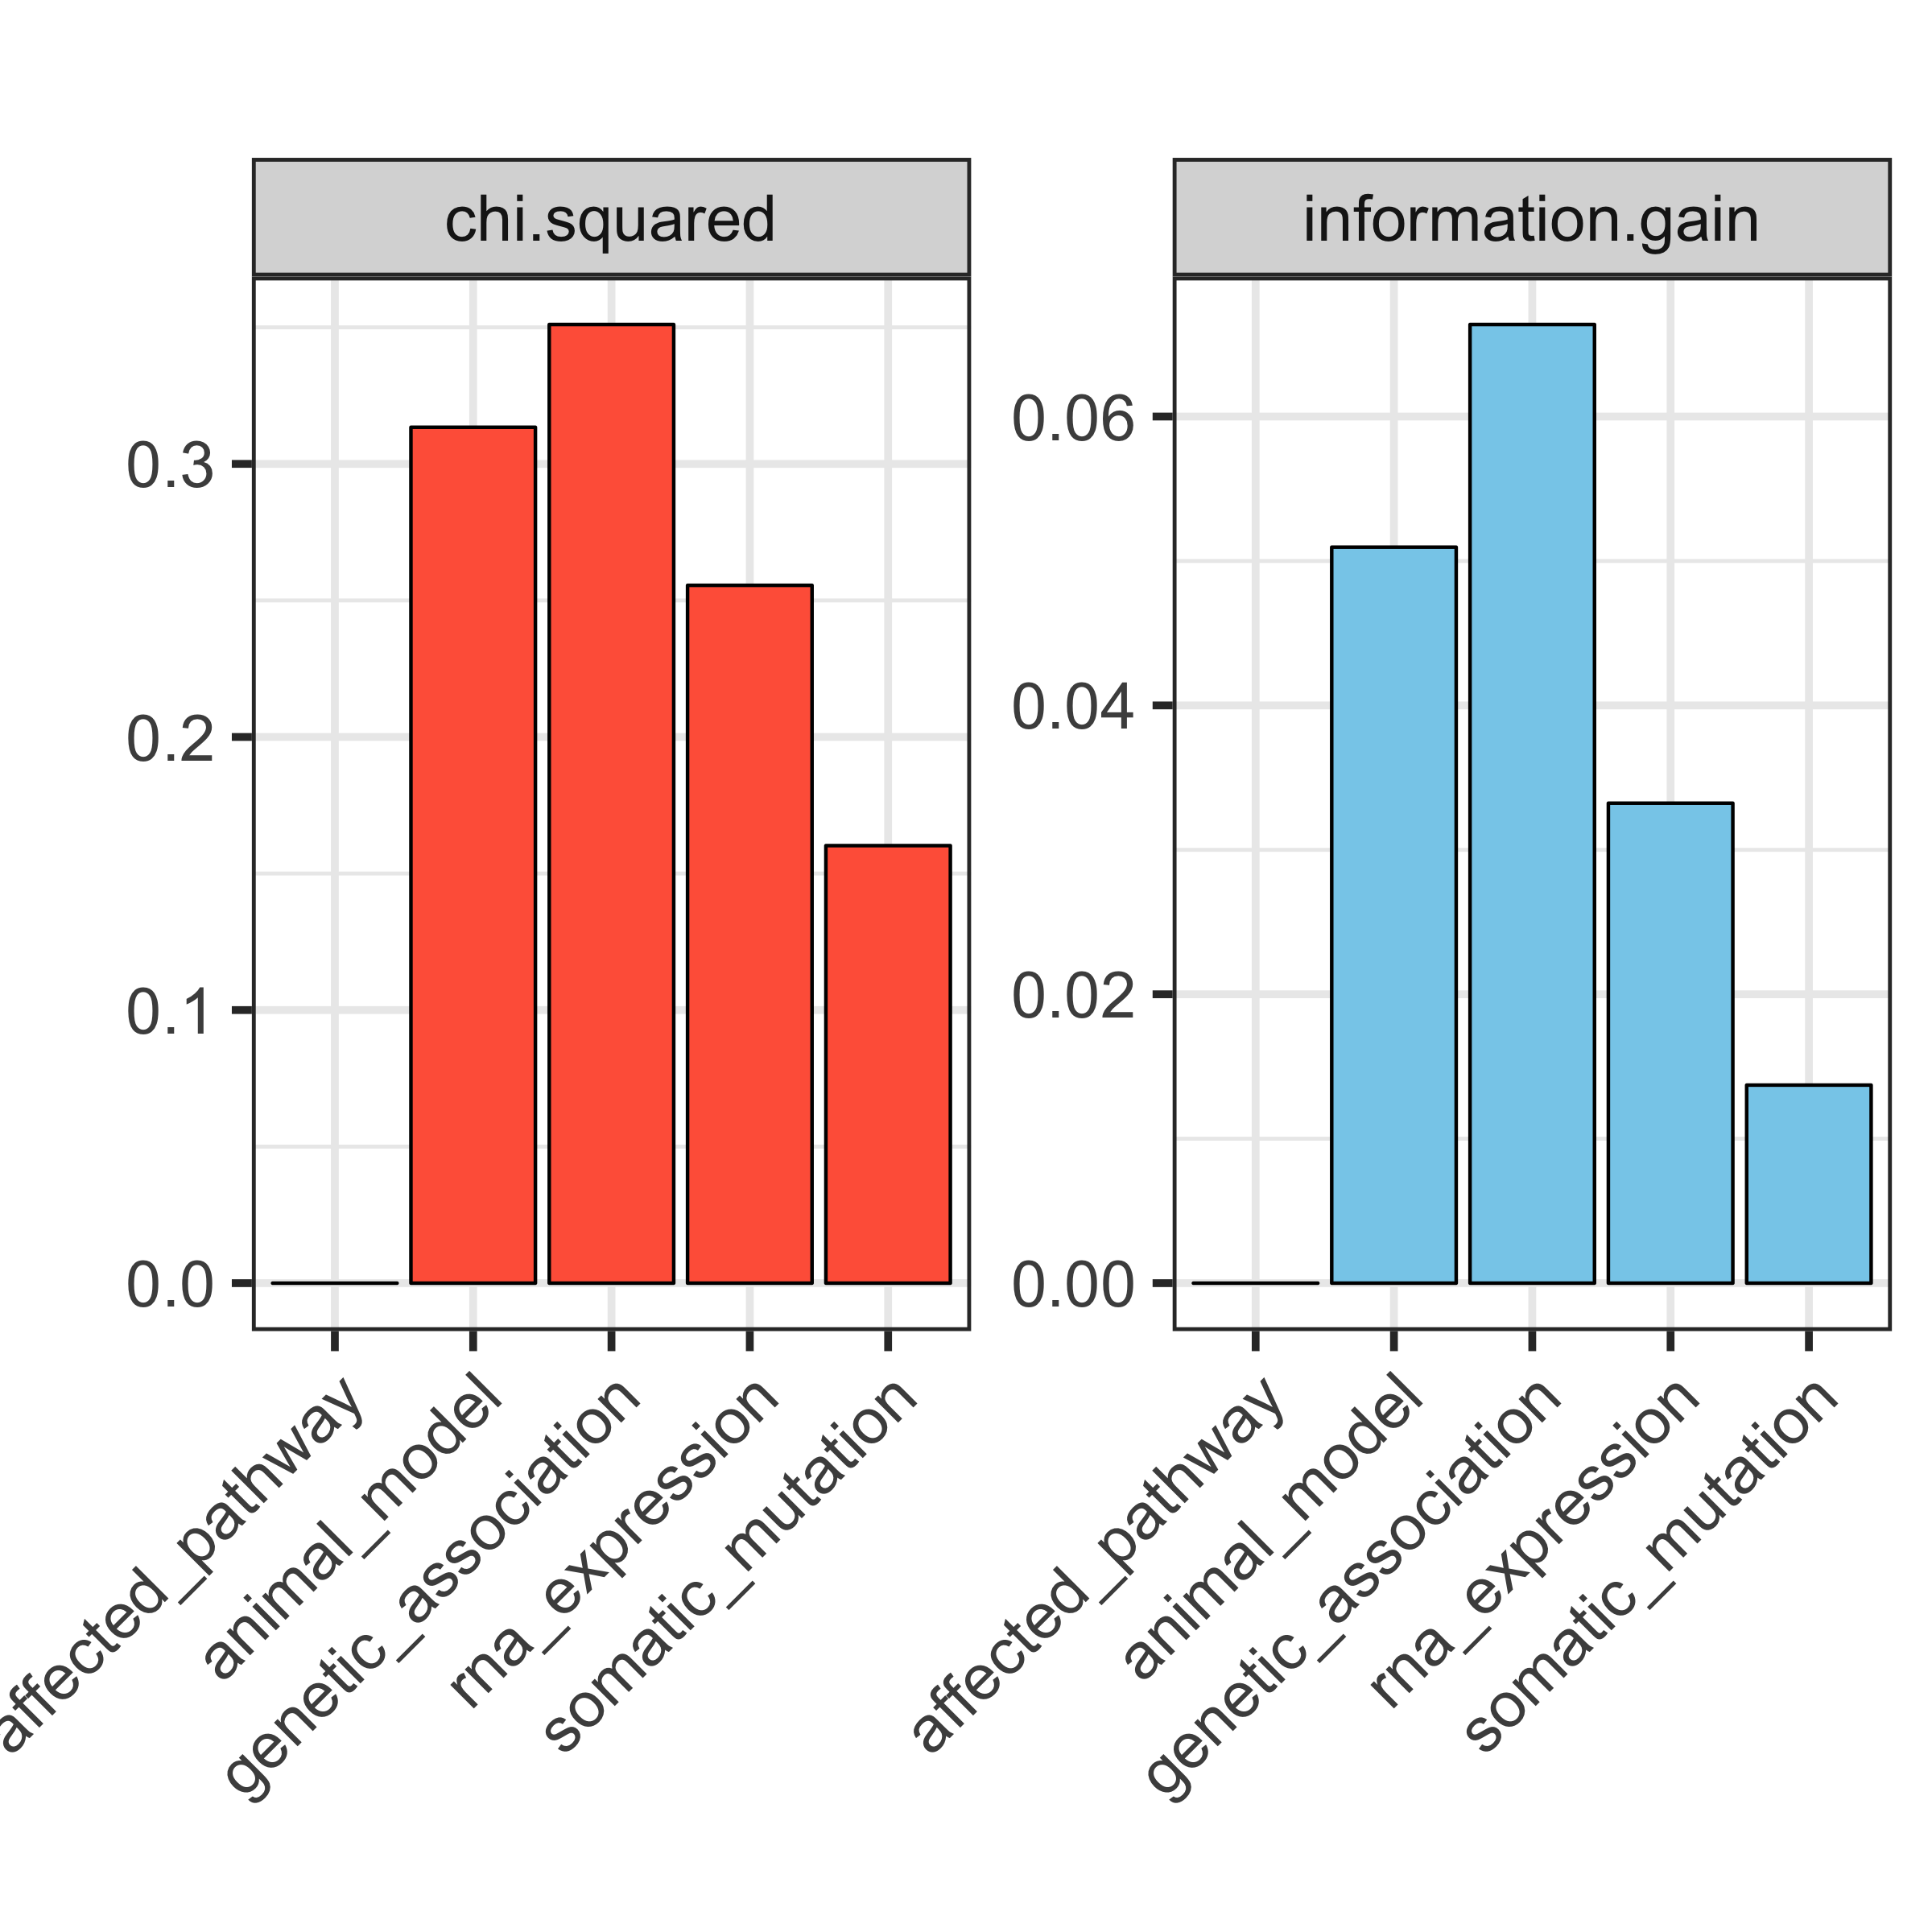
\includegraphics[width=78mm]{pics/Features.png}}
\hfill
\subfloat[Decision tree classification criteria: colours represent predicted outcome (purple: non-target, green: target). In each node, numbers represent (from top to bottom): outcome (FALSE: non-target, TRUE: target), number of observations in node per class (left non-target, right target), percentage of observations in node \label{fig:OT_decisionTree}]{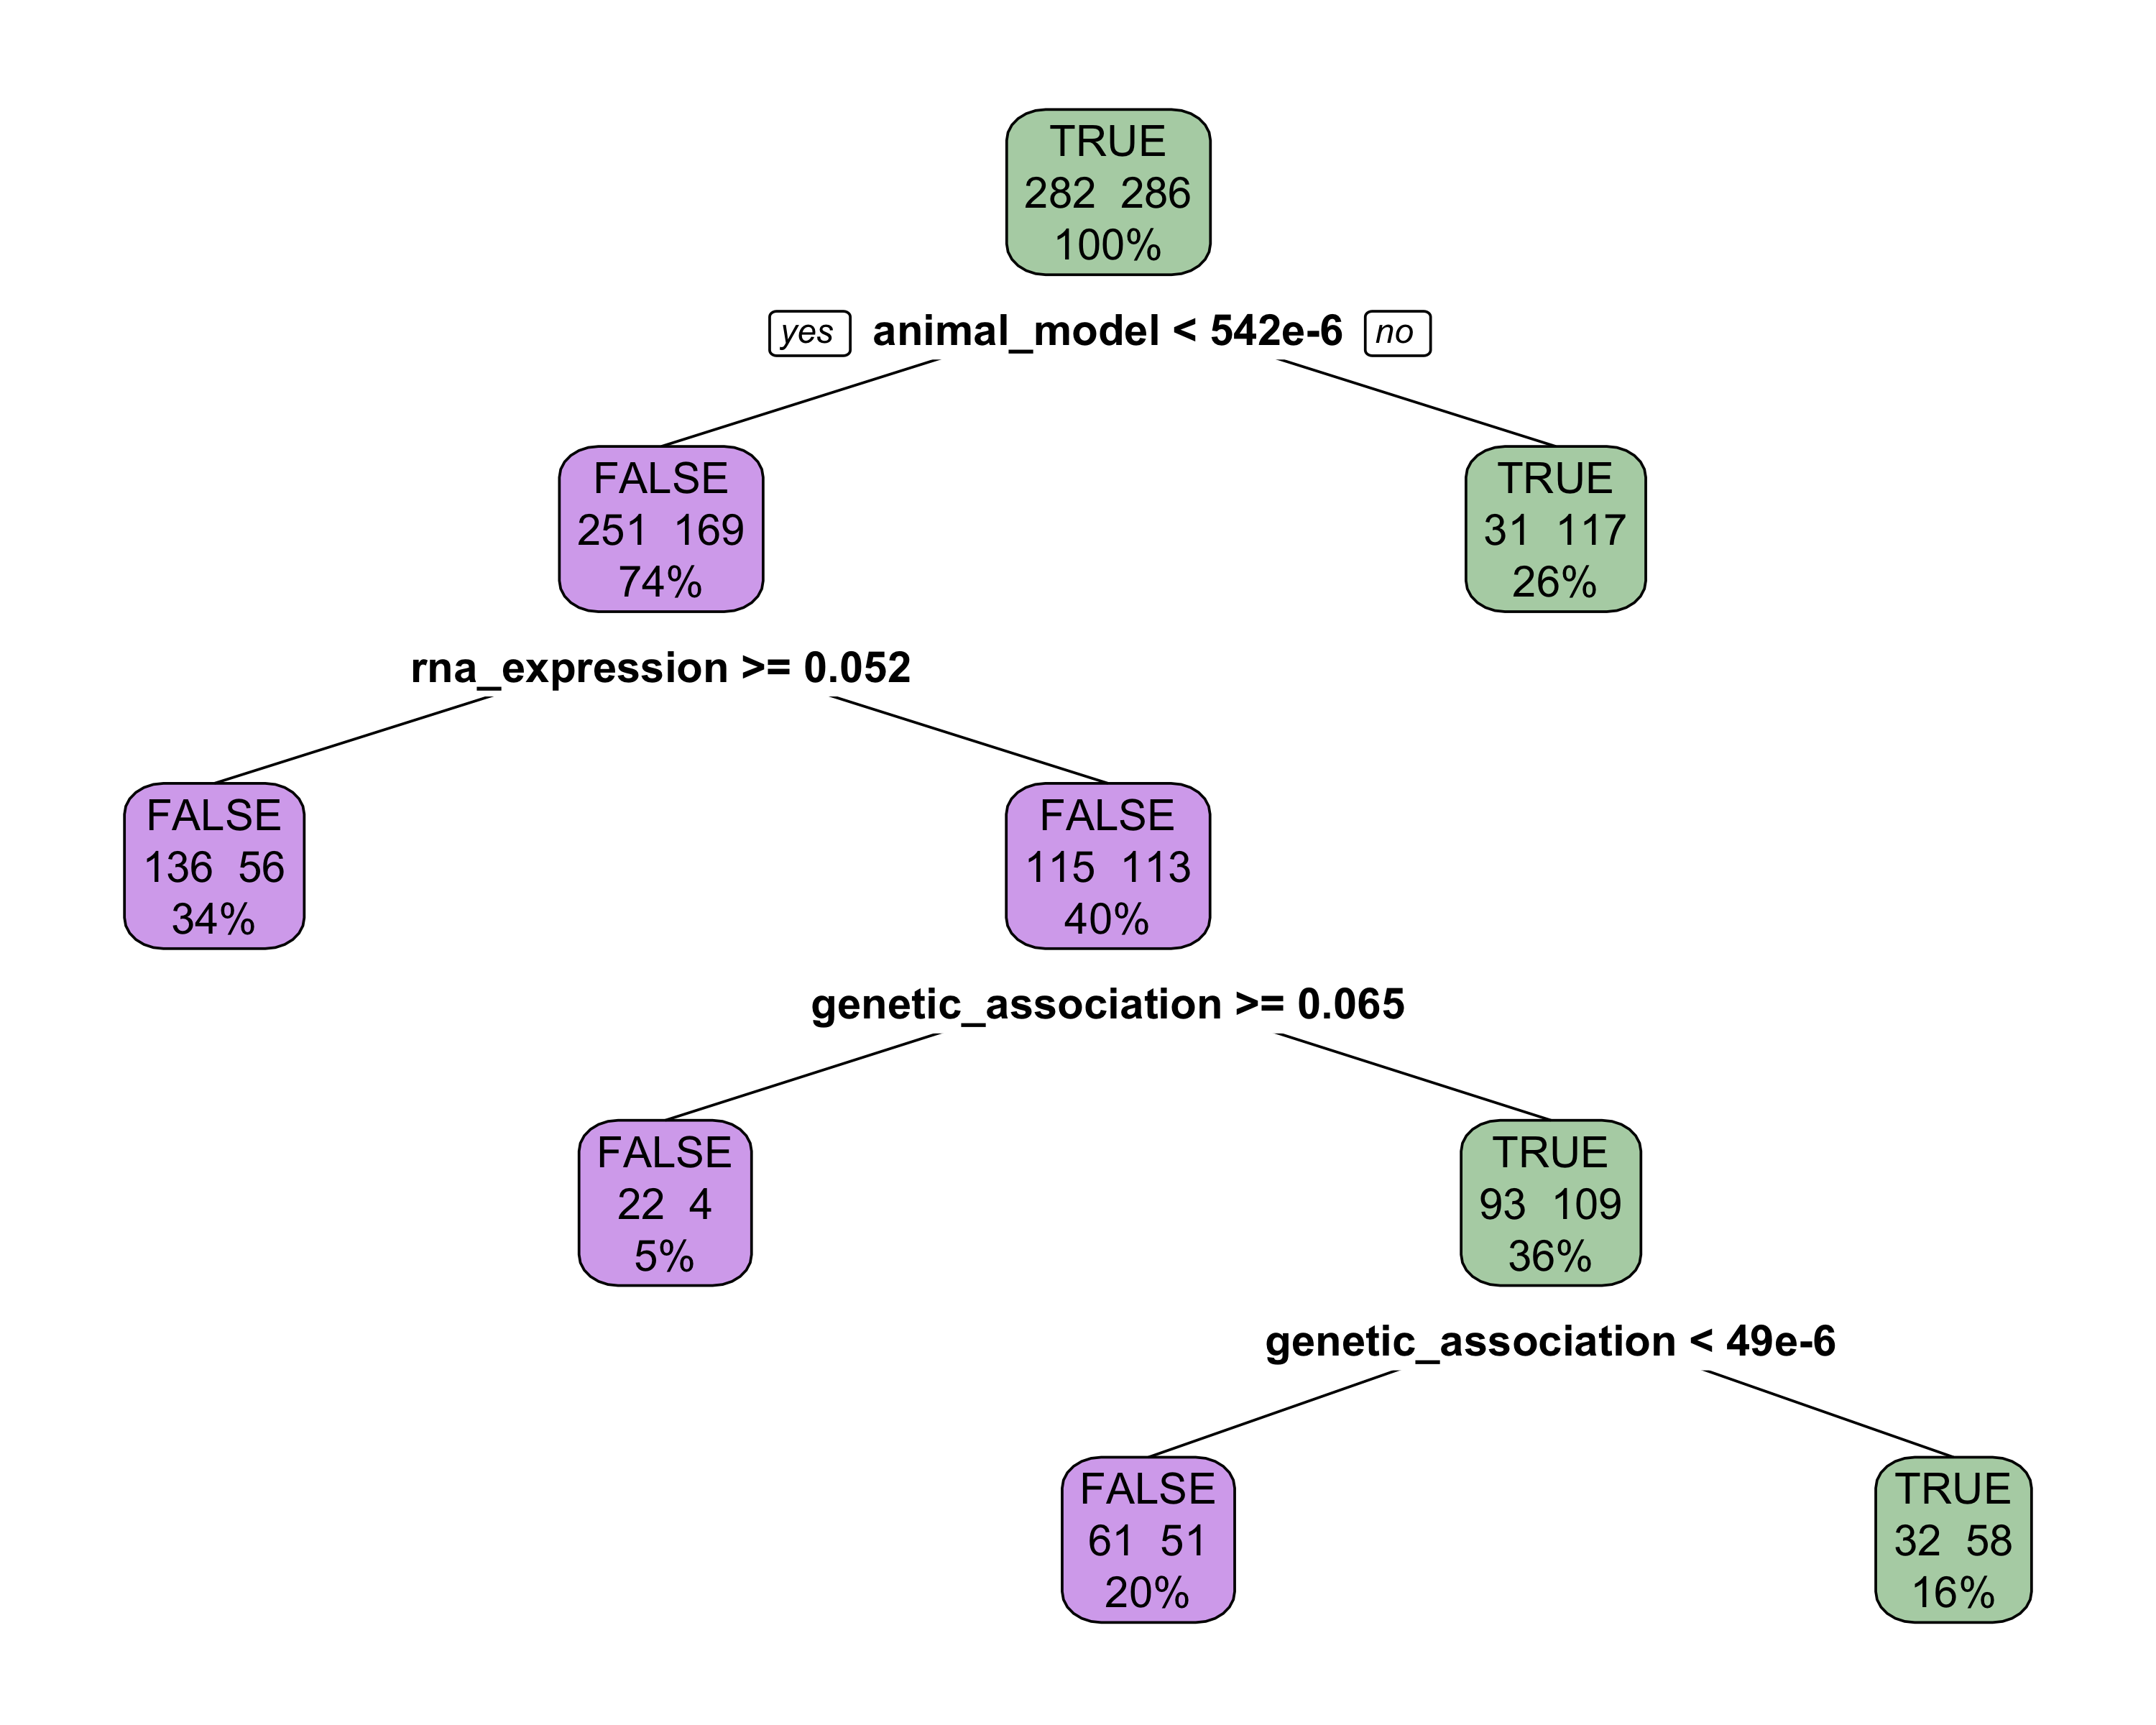
\includegraphics[width=78mm]{pics/DecisionTreeInf.png}}
\end{figure}

Four different classifiers were used, Random Forest (RF), Support Vector Machine (SVM), feed-forward Neural Network (NN) with a single hidden unit, and Gradient Boosting Machine (GBM) in a \emph{semi-supervised} approach on positive unlabelled data with \emph{nested cross-validation} (NCV). Some of the results of the classifiers are displayed in Figure \ref{fig:OT_OtherPlots}. Please refer to \href{https://github.com/davidnarganes/iCASErep}{GitHub repository} for the remaining results.

Why \textbf{semi-supervised}? Data was partially labelled and semi-supervised methods tackle problems when labelling of data is a limitant factor. Just the 8\% of all known human genes were known to be related to drugs. It is uncertain whether the remaining genes may become a potential target in the future \cite{ferrero2017}. 
    
Why \textbf{nested cross-validation} (NCV)? NCV generalises the estimation error of the model and its hyperparameters in an inner loop. Non-NCV biases the model yielding an overly optimistic score. A comparison between NCV and non-NCV in Python can be found \href{https://goo.gl/soHYT7}{elsewhere}.

\begin{figure}[H]
    \centering
    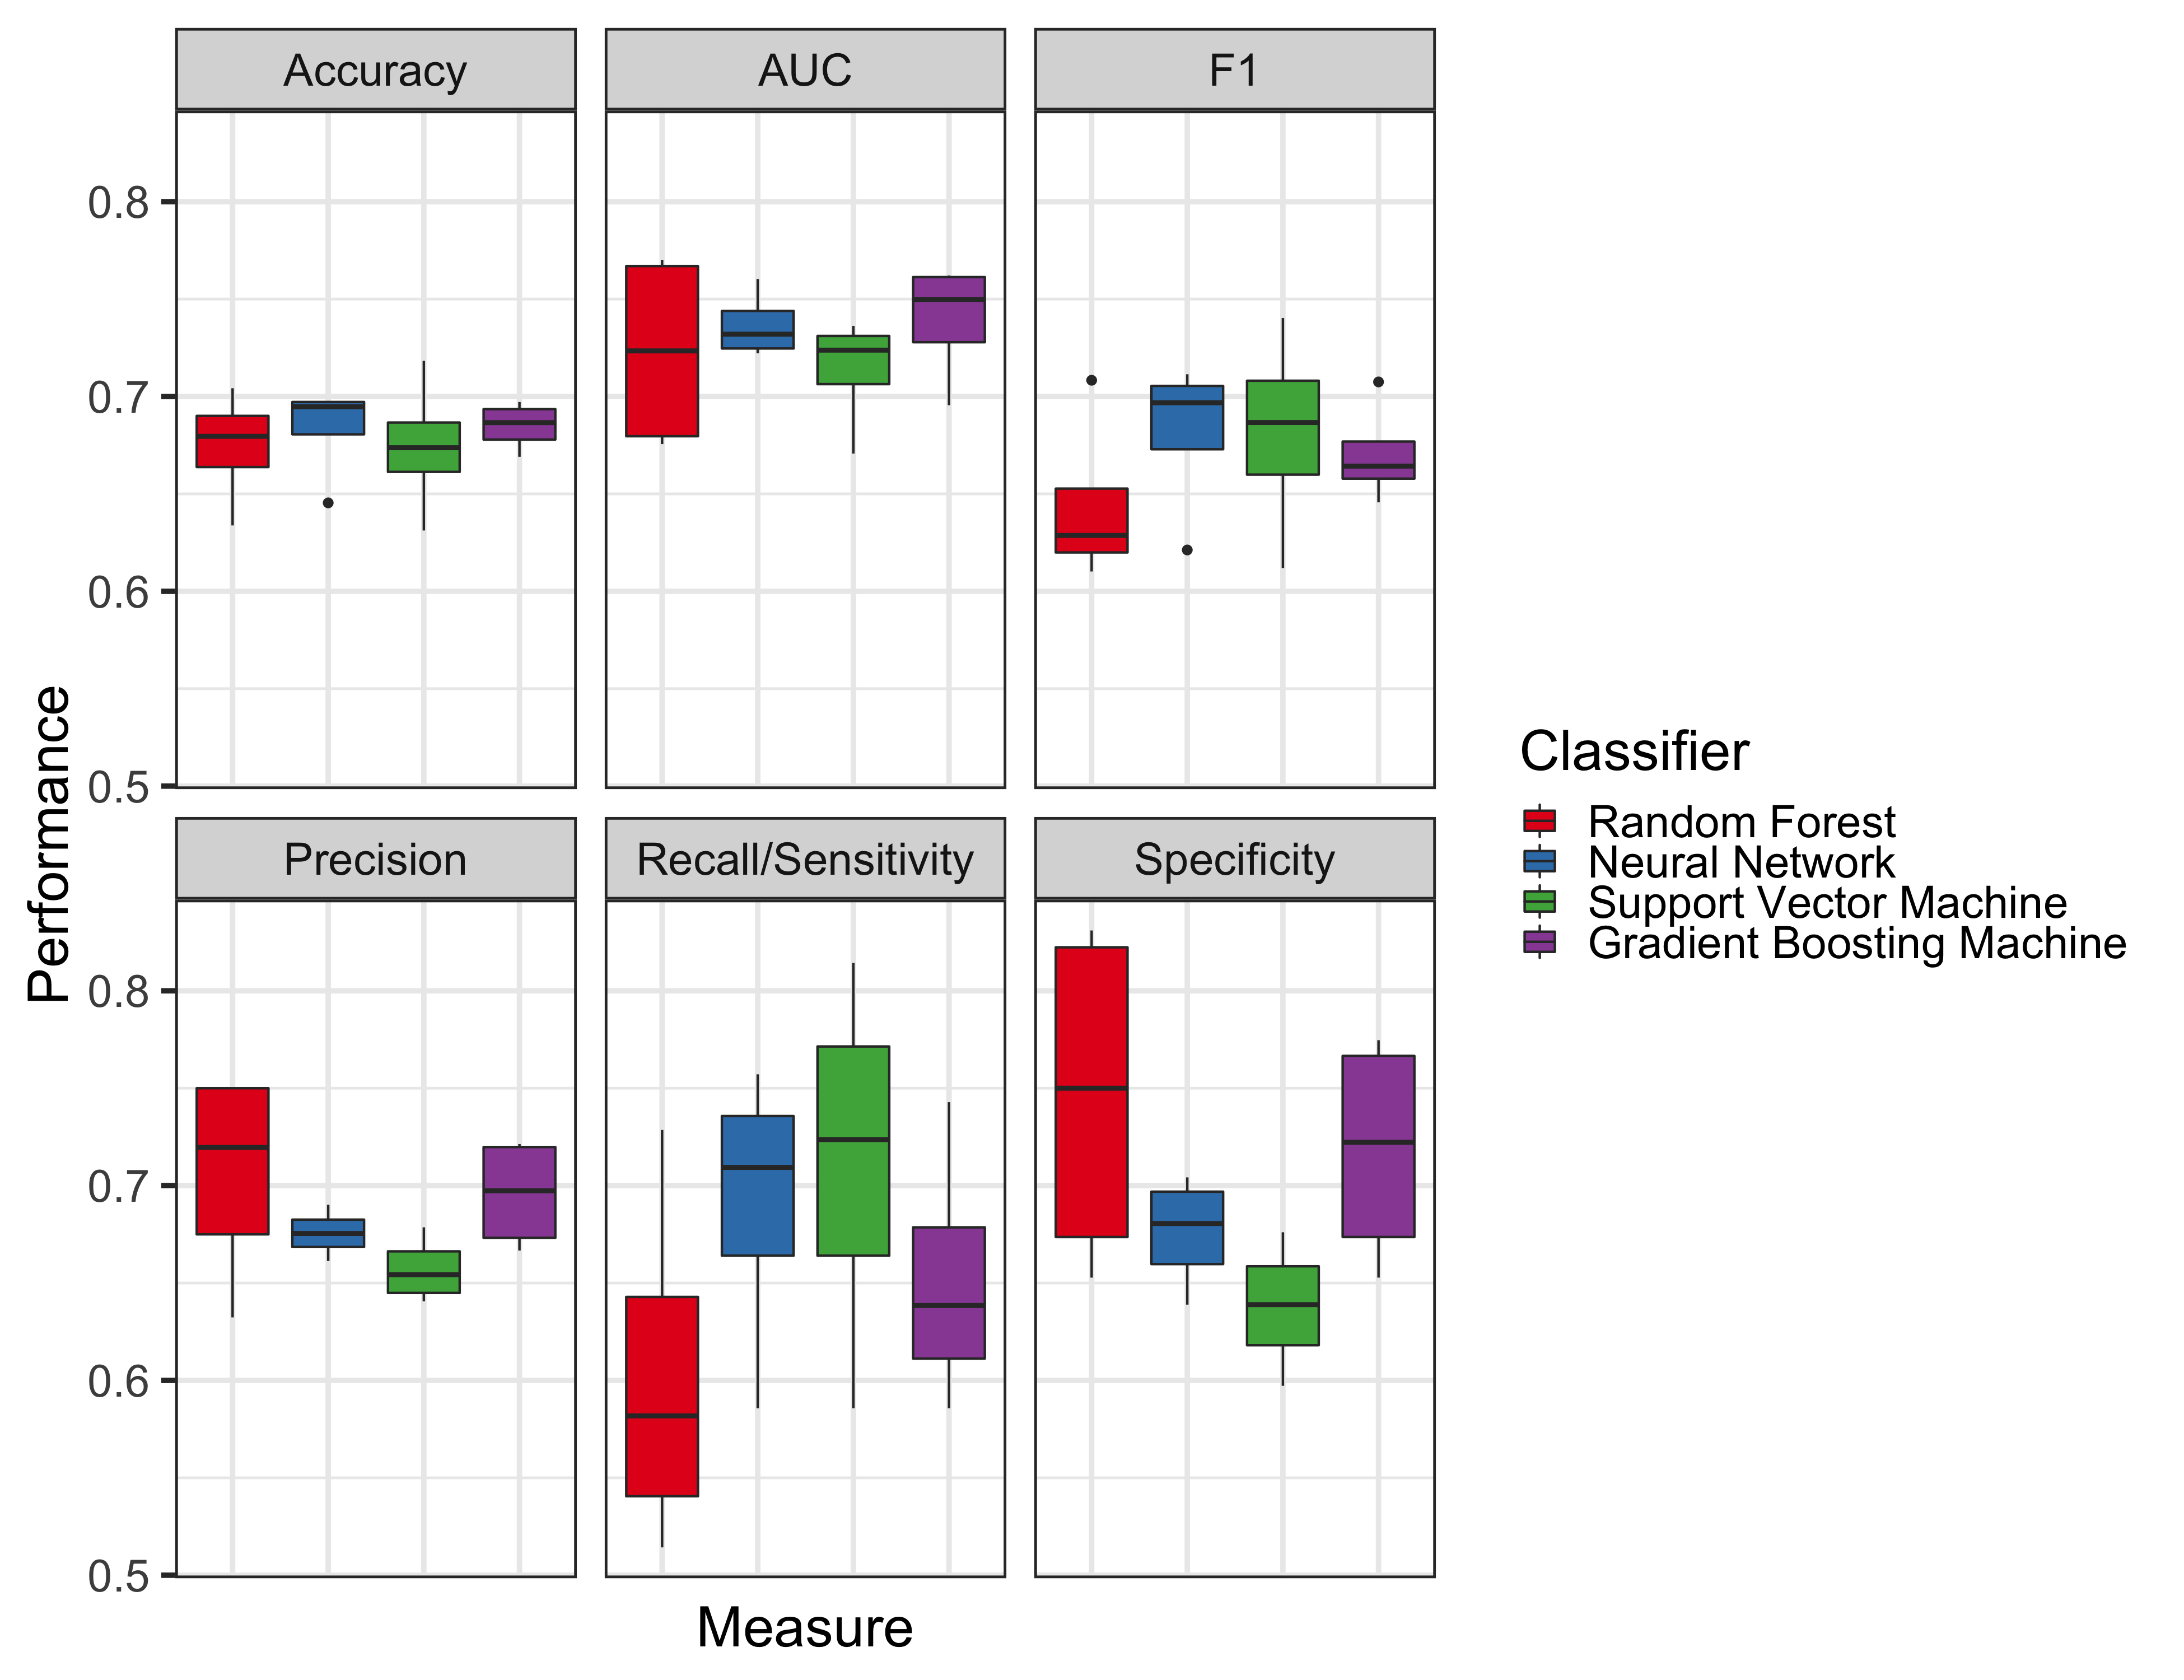
\includegraphics[width = 13cm]{pics/BenchmarkOtherBoxplots.png}
    \caption{Box plots showing distributions of the following measures for the four trained classifiers: accuracy, AUC, F1 measure, precision, recall/sensitivity and specificity, as assessed by NCV on the \texttt{training set} \label{fig:OT_OtherPlots}}
\end{figure}

Overall, all algorithms had comparable accuracy, AUC, and precision (see Figure \ref{fig:OT_OtherPlots}). These results are slightly lower than the ones reported by Ferrero et al. \cite{ferrero2017} (See my results in Table \ref{tab:David_perf_train_mean} and Ferrero's results in Table \ref{tab:OT_perf_train_mean}). 

\begin{table}[H]
\centering
\begin{tabular}{c|c|c|c|c|c|c|c}
Classifier & MMCE  & Accuracy   & AUC   & Recall/Sensitivity   & Specificity   & Precision   & F1    \\
\hline
RF & 0.326 & 0.674 & 0.723 & 0.602 & 0.746 & 0.705 & 0.644 \\
NN & 0.317 & 0.683 & 0.737 & 0.690 & 0.676 & 0.676 & 0.682 \\
SVM & 0.326 & 0.674 & 0.714 & 0.712 & 0.638 & 0.657 & 0.681 \\
GBM & 0.315 & 0.685 & 0.739 & 0.651 & 0.718 & 0.696 & 0.670
\end{tabular}
\caption{\textbf{David results}. Mean \texttt{training set} performance measures (mean misclassification error, mean accuracy, mean AUC, mean recall/sensitivity ratio, mean specificity, mean precision, mean F1 measure) for all classifiers estimated by NCV \label{tab:David_perf_train_mean}}
\end{table}

\begin{table}[H]
\centering
\begin{tabular}{c|c|c|c|c|c|c|c}
Classifier & MMCE  & Accuracy   & AUC   & Recall/Sensitivity   & Specificity   & Precision   & F1    \\
\hline
RF         & 0.302 & 0.698 & 0.761 & 0.596 & 0.802 & 0.753 & 0.665 \\
NN         & 0.303 & 0.697 & 0.758 & 0.610 & 0.785 & 0.742 & 0.670 \\
SVM        & 0.317 & 0.683 & 0.733 & 0.592 & 0.775 & 0.729 & 0.652 \\
GBM        & 0.297 & 0.703 & 0.752 & 0.637 & 0.771 & 0.738 & 0.683
\end{tabular}
\caption{\textbf{Open Targets \cite{ferrero2017}}. Mean \texttt{training set} performance measures (mean misclassification error, mean accuracy, mean AUC, mean recall/sensitivity ratio, mean specificity, mean precision, mean F1 measure) for all classifiers estimated by NCV \label{tab:OT_perf_train_mean}}
\end{table}

The overlap in the classification is reported in Figure \ref{fig:OT_venn}.

\begin{figure}[H]
\resizebox{\textwidth}{!}{
    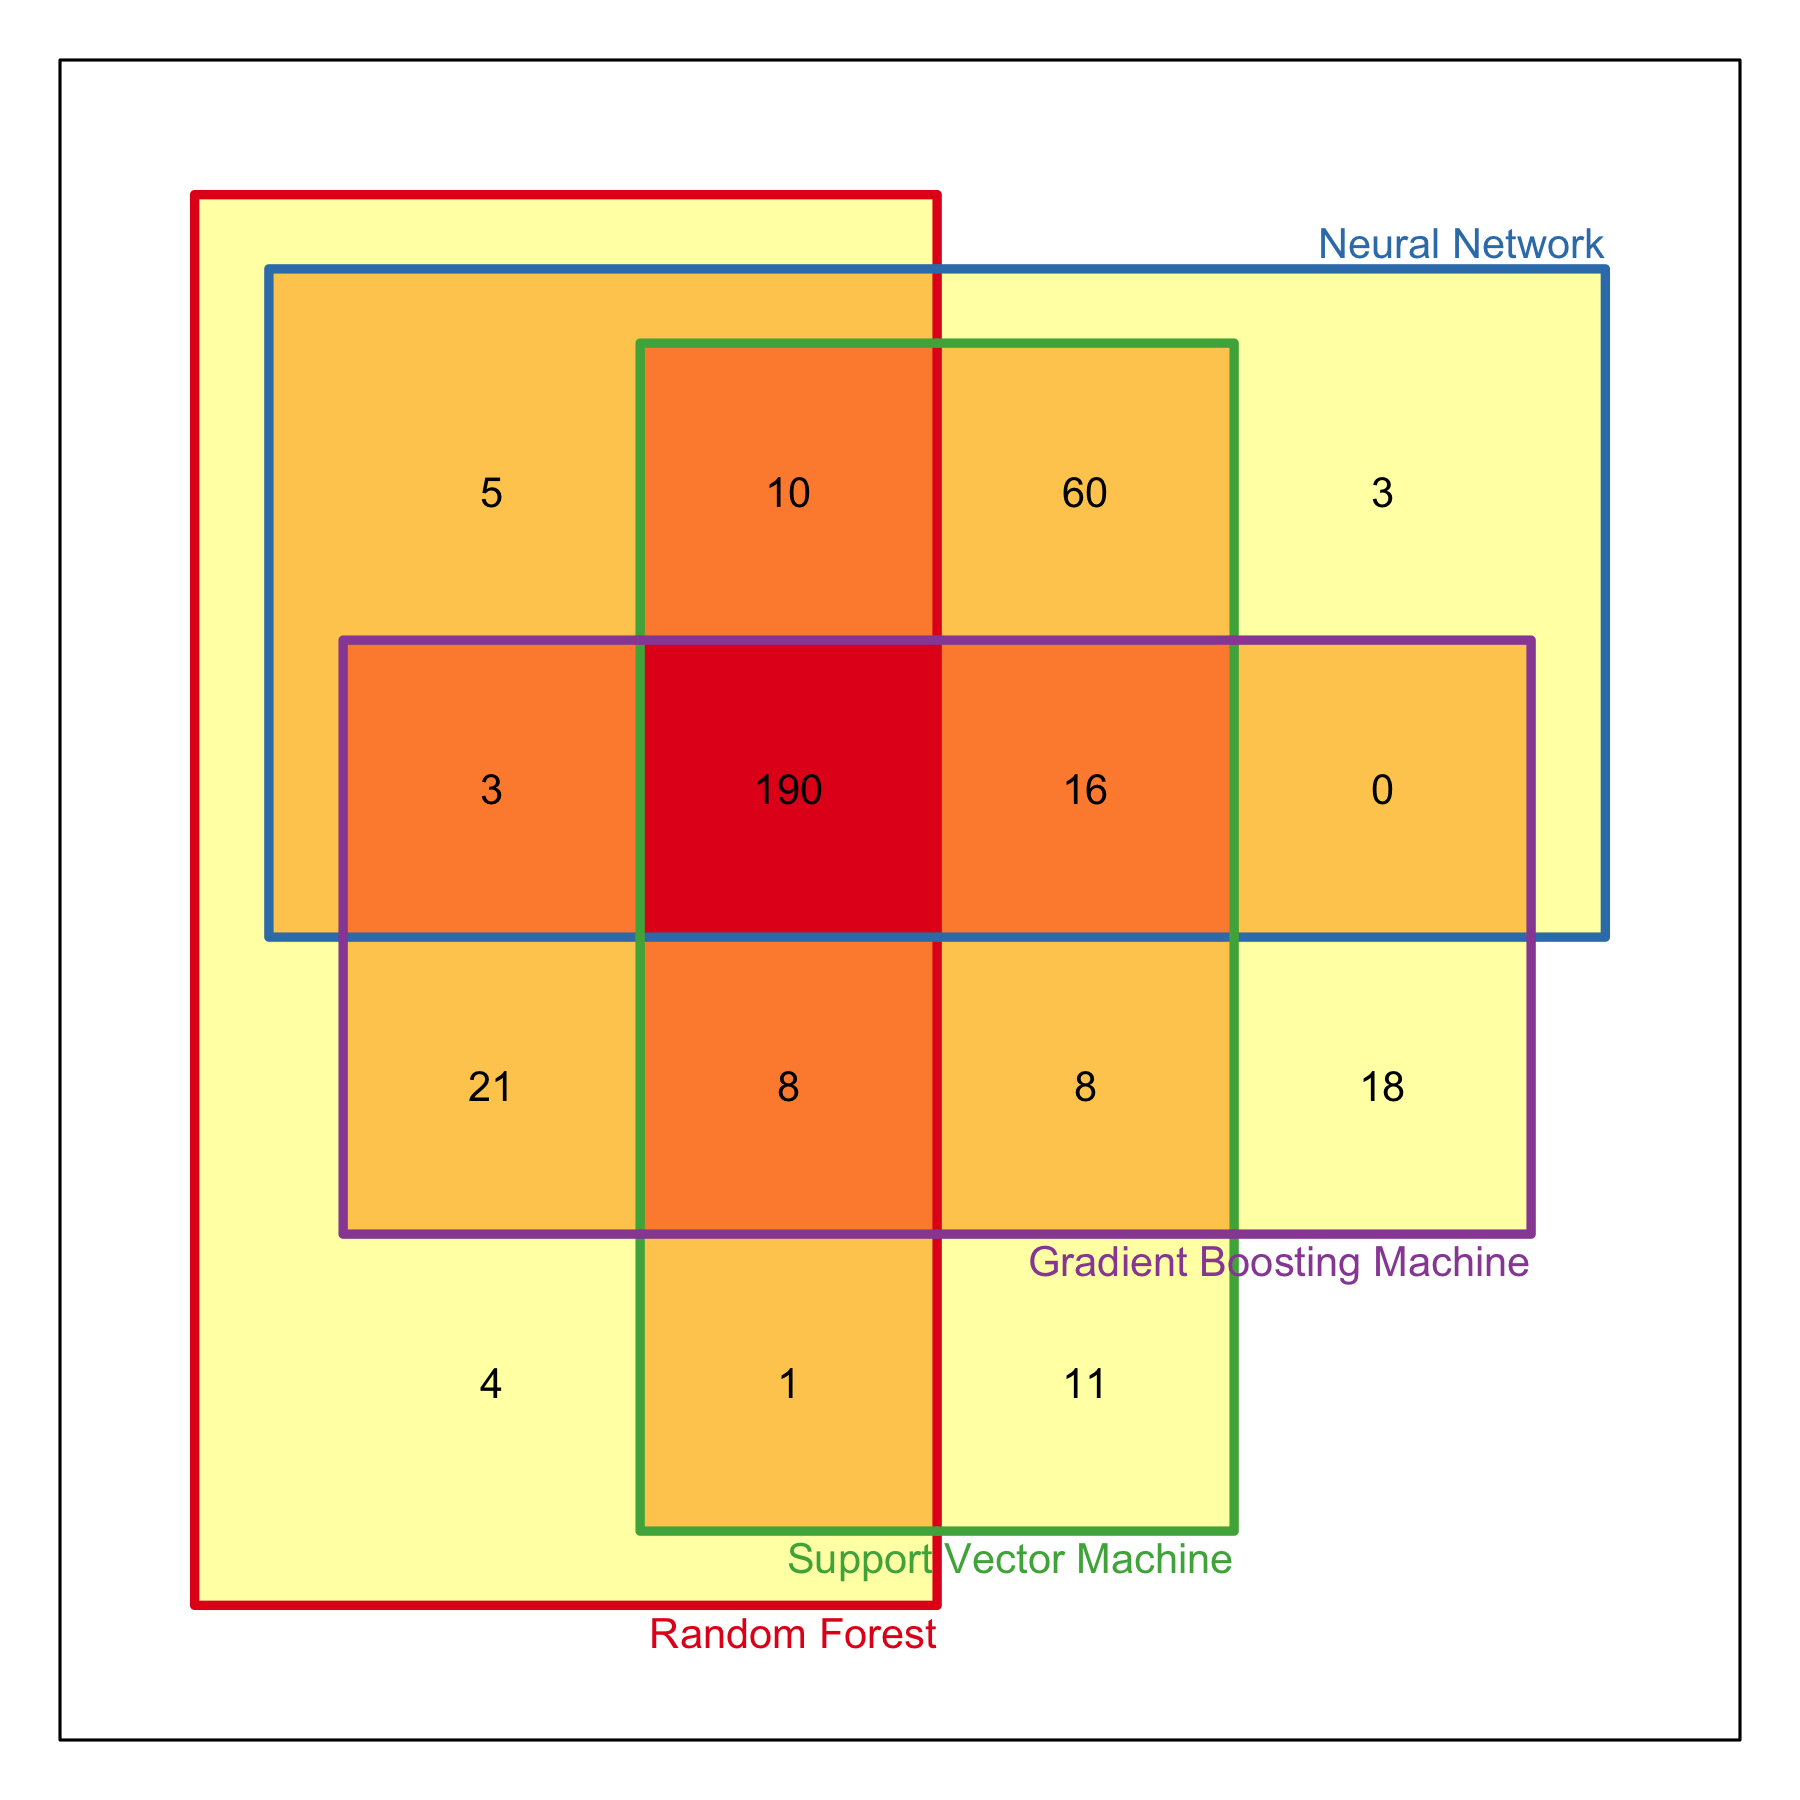
\includegraphics{pics/VennTargets.png}
    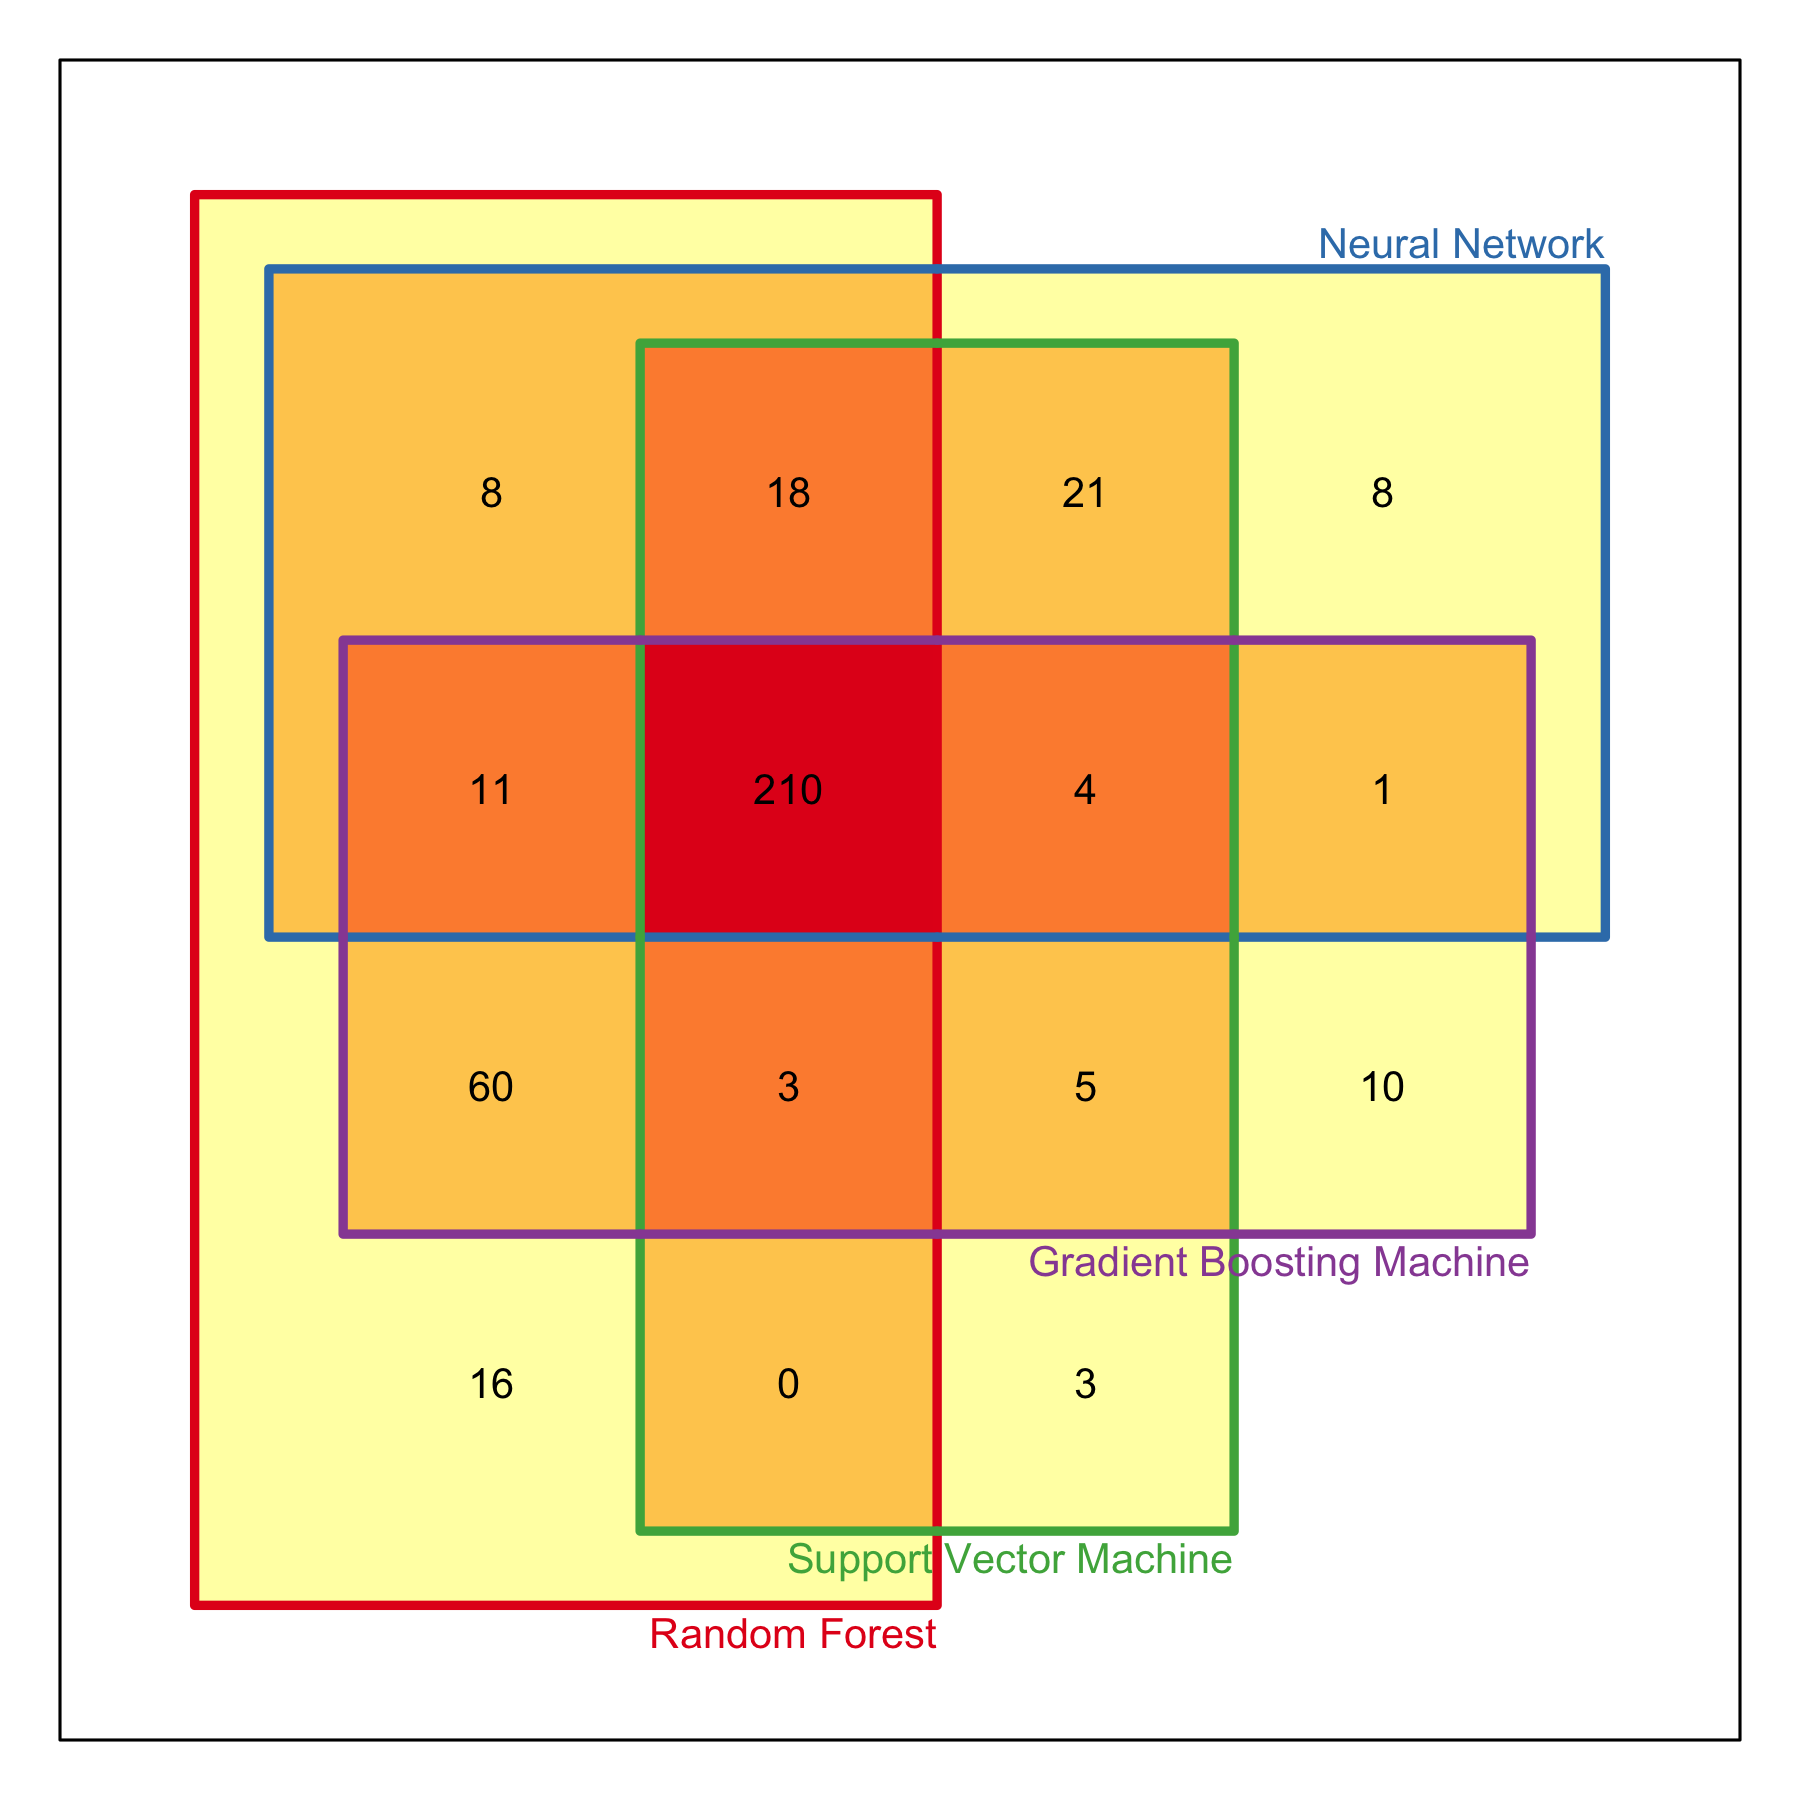
\includegraphics{pics/VennNontargets.png}}
    \caption{Overlap of predicted targets across the four trained classifiers. Venn diagrams showing the relative overlap of predicted targets (left) and predicted non-targets (right) from the \texttt{training set} for the four trained classifiers \label{fig:OT_venn}}
\end{figure}

\subsubsection{Limitations}
\label{subsub:limitations_openTargets}
\begin{enumerate}
    \item \textbf{Labelling of the classes}: there is no pure negative nor positive class which complicates the problem of a binary classification. Nonetheless, defining \emph{bona fide} unsuccessful targets is extremely difficult, if possible at all.
    
    Ferrero et al. \cite{ferrero2017} stated that the unlabelled, negative set contained both future positive targets but from an algorithmic perspective, they simply treated the unlabelled data as the negative set. For this reason, the number of true positives will be  underestimated \cite{ferrero2017}.
    
    Some drugs in early stages of drug development were defined as \emph{positive} successful targets but they may fail in latter stages.
    
    \item The best classifier, the NN, had a poor 71\% accuracy.
    
    \item  Inclusion of functional (Gene Ontology, pathways), structural (protein domains) or interaction data (protein-protein interactions) is likely to have a large impact on the ability to successfully predict targets.
    
    \item Their predictions were individual targets, and not target-disease pairs.
    
    \item Ferrero et al. did not make any claim regarding the druggability of these targets. Open Targets answers questions focused on GDAs but is unable to report focused aspects about the bioactivity profiles of small molecules on those targets \cite{brown2018}
    
    \item Ferrero et al. removed the feature \texttt{literature} since it it was likely to be heavily biased towards well known, validated target–indication pairs. What about \texttt{animal\_model}? Why \texttt{animal\_model} is a good feature for predicting \textbf{novel} therapeutics? The feature \texttt{animal\_model} is a proxy of how much time, research, and money has been spent on a target. Furthermore, their models predicted better later stage targets \cite{ferrero2017}.
    
    \item They claimed that their data types report characteristics that makes good therapeutic targets \cite{ferrero2017} but the main feature is \texttt{animal\_model}. There is no causality, just correlation. The fact of making an experiment about one target on animals does not make that target good. Researchers and companies do not invest money on random targets.
\end{enumerate}